% encoding: utf8
% !TEX encoding = utf8
% !TeX spellcheck = pl_PL


\documentclass[12pt,a4paper]{article}
\usepackage[margin=0.8in]{geometry}
\usepackage{amsmath}
\usepackage{amssymb}
\usepackage[english,polish]{babel}
\usepackage{cite}
\usepackage{graphicx}
\usepackage{hyperref}
\usepackage[utf8]{inputenc}
\usepackage{listings}
\usepackage{polski}
\usepackage{url}
\usepackage{float}
\usepackage[nottoc]{tocbibind}


\graphicspath{ {./images/} }


\lstset{
	basicstyle=\ttfamily,
	columns=fullflexible,
	frame=single,
	breaklines=true,
	postbreak=\mbox{{$\hookrightarrow$}},
}


\begin{document}
	\title{Pracownia dyplomowa magisterska \\ Sterowanie ramieniem robota w obliczu chwytania przedmiotów}
	\author{Jakub Postępski}
	\maketitle


	\section{Wprowadzenie}
	Celem tej pracy magisterskiej jest rozwiązanie problemu kompensacji grawitacji w ramieniu robota sterowanym impedancyjnie. Zakłada się nieznany model chwytanego obiektu, znany model ramienia robota oraz nieważkość ramienia robota. Zakładamy dostępność pomiarów z nadgarstkowego czujnika siły i momentu. W trakcie wspomnianej kompensacji grawitacji robot nie powinien tracić swoich zalet związanych z tym typem sterowania. Dodatkowo ramię robota zakończone jest chwytakiem który pozwala na chwytanie przedmiotów.

	Środowiskiem badawczym jest robot Velma\cite{velma} (rys. \ref{fig:velma}). Ma on dwa ramiona LWR\cite{lwr} sterowane impedancyjnie. Posiadają wbudowaną kompensację grawitacji własnej masy. Na ich końcach znajdują się chwytaki Barretta oraz nadgarstkowe czujniki FTS.

	\begin{figure}[H]
		\centering
		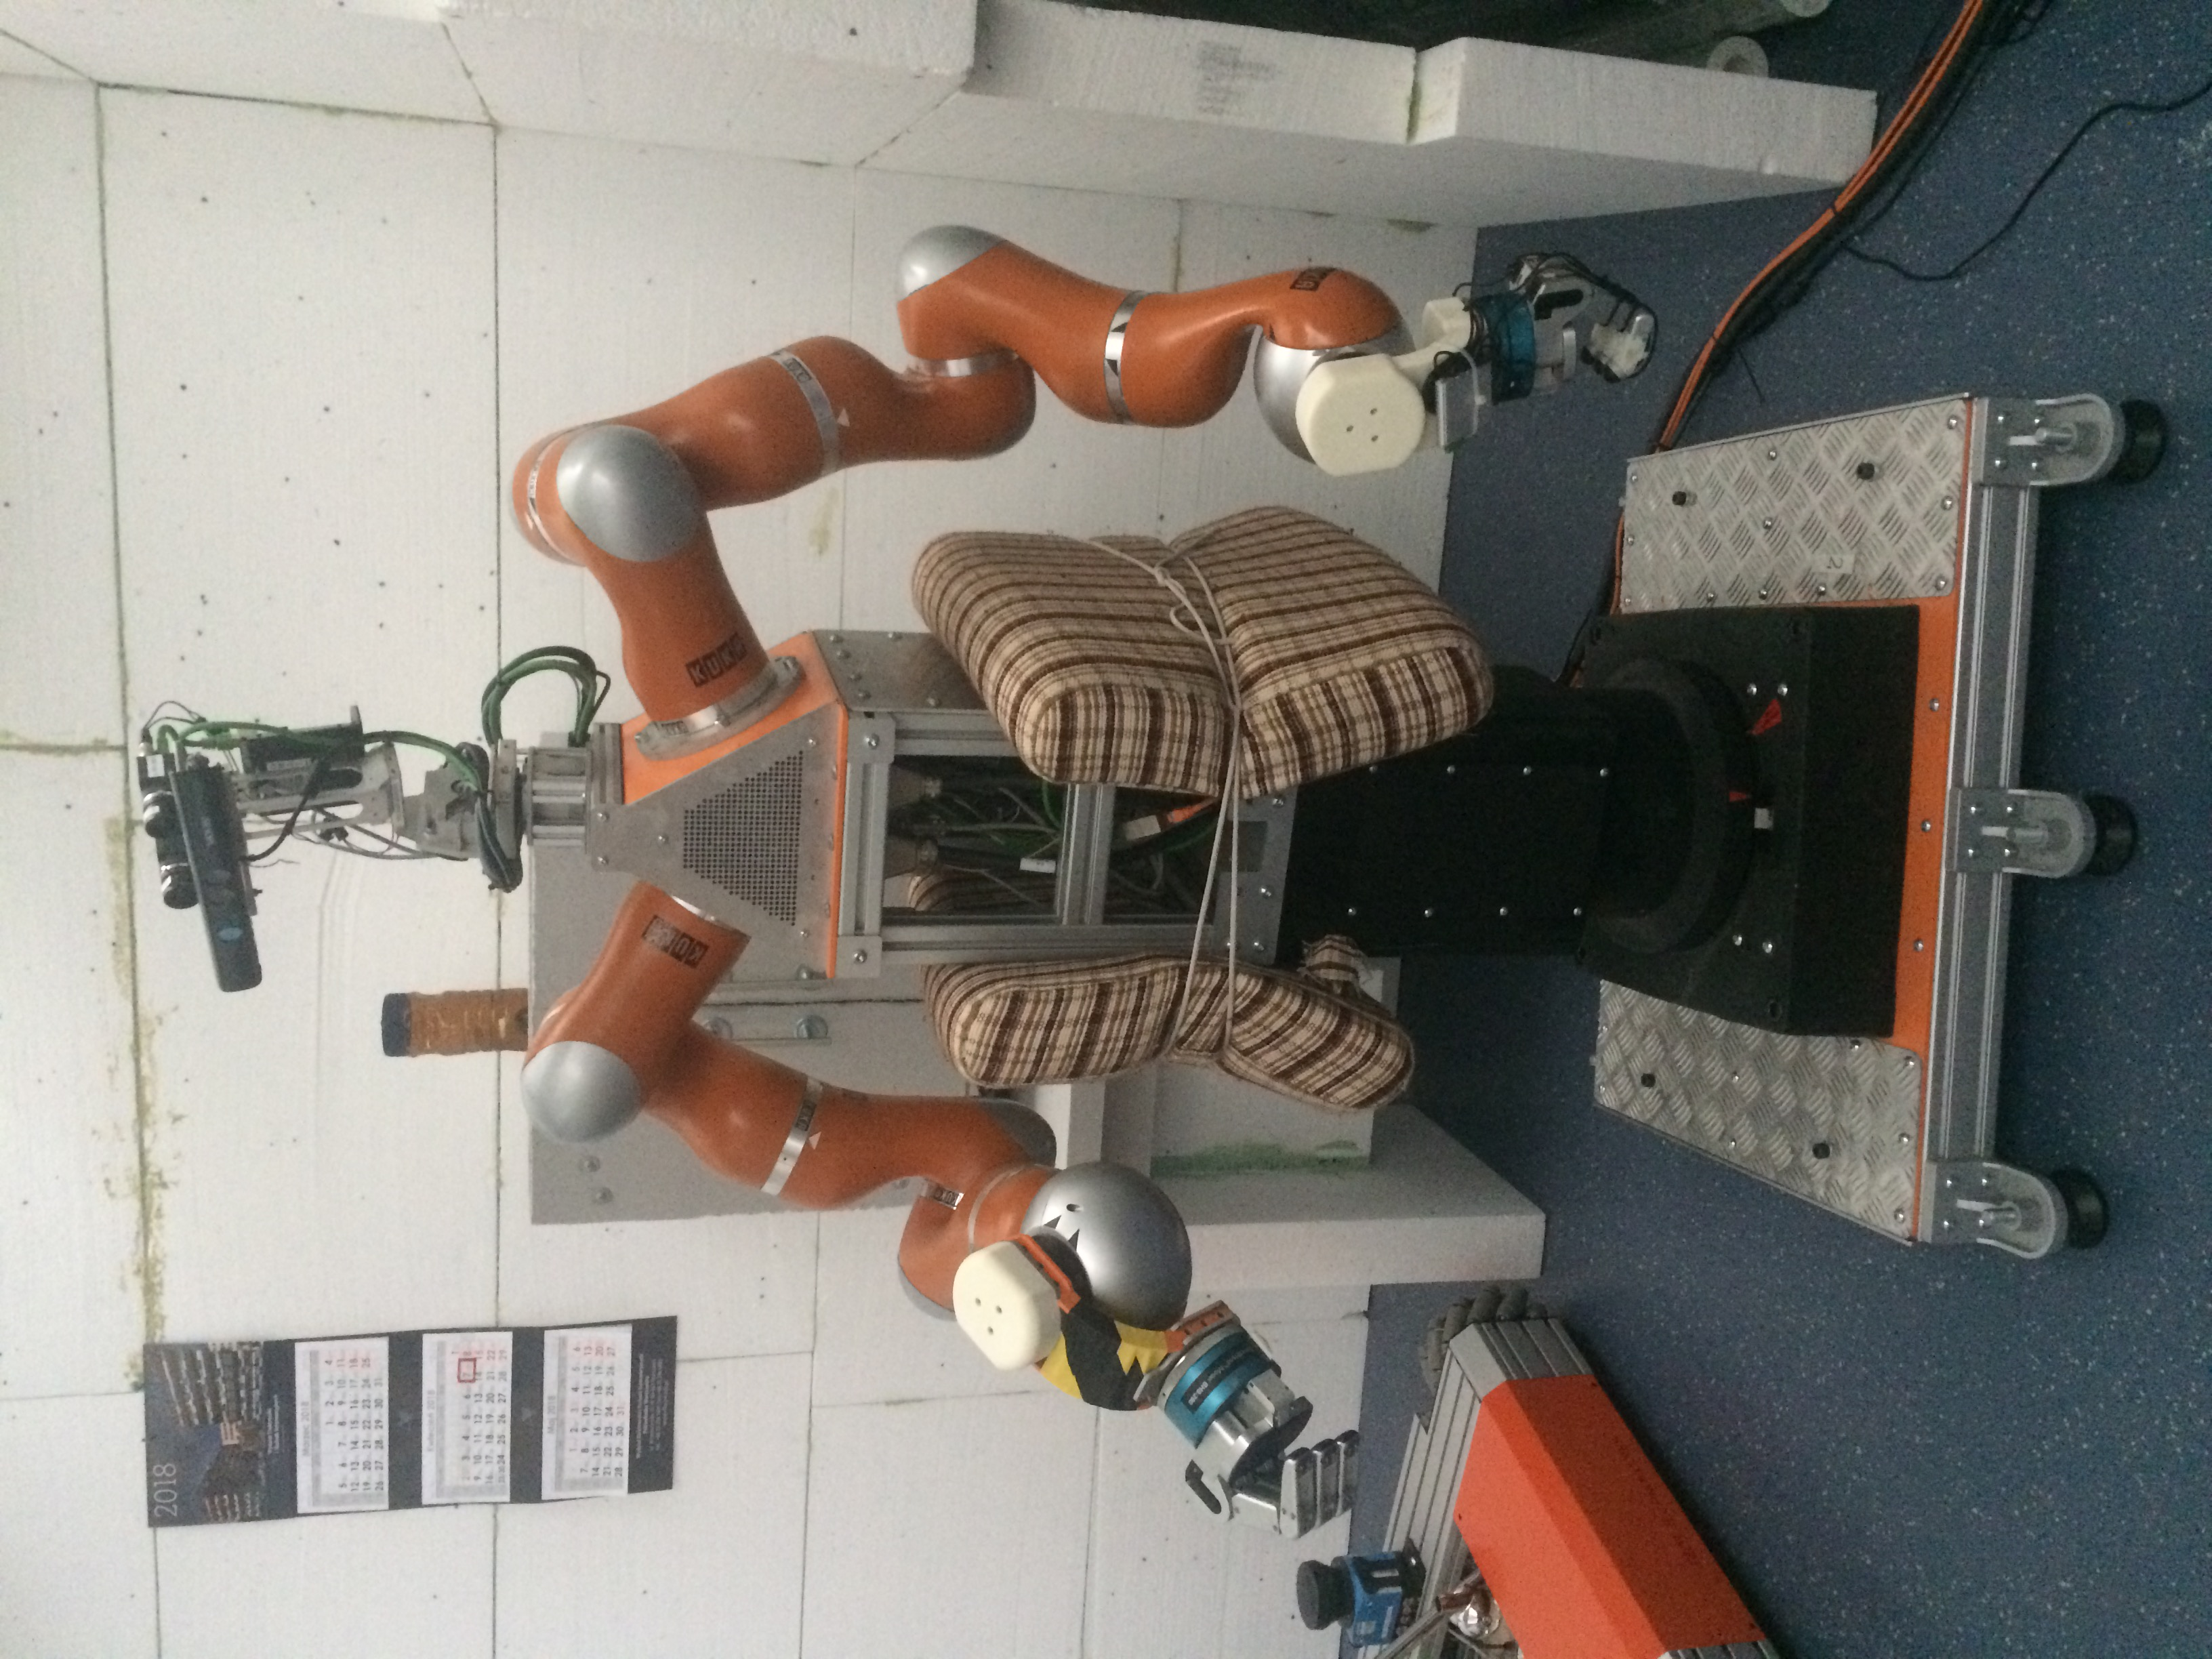
\includegraphics[scale=0.05, angle =-90]{velma}
		\caption{Robot usługowy Velma}
		\label{fig:velma}
	\end{figure}

	System sterowania o twardych ograniczeniach czasowych pracuje z częstotliwością 500 Hz. Struktura oprogramowania (rys. \ref{fig:agenty}) została stworzona w oparciu o teorię agentową. Agent \textbf{velma\_core\_cs} jest odpowiedzialny za kontrolę zadań związanych z manipulacją w przestrzeni operacyjnej i konfiguracyjnej robota poprzez kontrolę efektorów i receptorów robota. Agent \textbf{velma\_ros\_interface} służy do kontroli i interpretacji zadań zleconych przez użytkownika poprzez zarządzanie agentem \textbf{velma\_core\_cs}. Oprogramowanie agenta \textbf{velma\_core\_cs} jest wykonane przy wykorzystaniu struktury ramowej Orocos, natomiast agenta \textbf{velma\_ros\_interface} przy użyciu struktury ramowej ROS. Dostępny jest też symulator robota pisany w przy wykorzystaniu Gazebo. Do obserwowania pracy poszczególnych komponentów systemu służy narzędzie rqt\_agent.

	\begin{figure}[H]
		\centering
		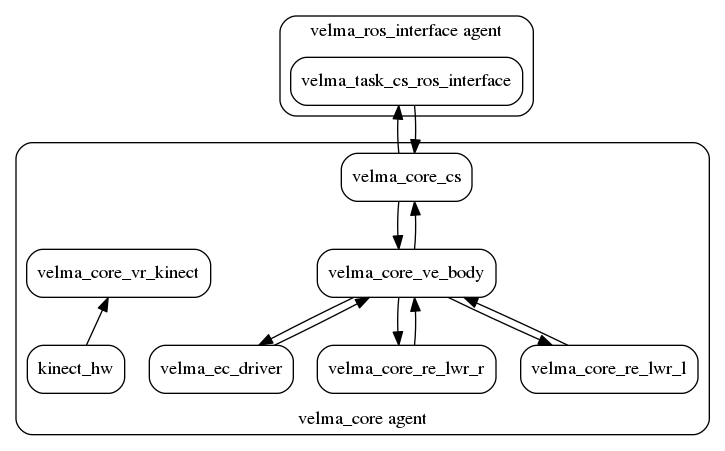
\includegraphics[width=0.8\linewidth]{agenty}
		\caption{Agentowa struktura oprogramowania \cite{velma}}
		\label{fig:agenty}
	\end{figure}

	\section{Poszerzanie wiedzy}
	\subsection{Artykuły}
	Artykuł \cite{impedance} pozwala na zrozumienie podstaw sterowania impendancyjnego dla ramion robotów. Artykuły \cite{gravity1} i \cite{gravity2} przedstawiają przykładowe rozwiązania problemu kompensacji grawitacji.

	Na wykładach z Teorii sterowania można uzyskać wiedzę na temat podstawowych struktur sterowania. Poruszane są problemy systemów z czasem dyskretnym. Omawiane są problemy konstrukcji optymalnych estymatorów regulatorów i obserwatorów. Jeden z wykładów poświęcony został regulacji adaptacyjnej. Omawiane są zagadnienia niwelowania szumów znajdujących się w układzie. 	Na przedmiocie Algorytmy i metody optymalizacji poruszana jest tematyka optymalizacji funkcji liniowych i nieliniowych z ograniczeniami. Omawiany jest problem sprowadzania optymalizacji funkcji nieliniowej i niewypukłej do prostszych postaci. Prezentowane są szybkie algorytmy optymalizacji funkcji kwadratowych. W ramach wykładów z  Modelowania i sterowania robotów omawiane są zagadnienia opisu kinematyki i dynamiki robotów. Na przedmiocie Inteligentne systemy robotyczne omawiane są zagadnienia teorii agentowej i zastosowania tej teorii w robotyce.

	Uczęszczanie na wykłady oraz czytanie artykułów pozwoliło na wyrobienie ogólnego poglądu na przedstawiony problem. Szczególnie istotne była zdobyta wiedza na temat optymalnych regulatorów i obserwatorów. Ważne okazały się też metody optymalizacji ponieważ mogą pozwolić na sprawną implementację wymienionych narzędzi.


	\section{Model chwytanego przedmiotu}
	Obiekt można identyfikować przetwarzając dane z czujnika FTS. W eksperymencie prowadzonym w trakcie ruchu należy uwzględnić siłę bezwładności. Wprowadza to dodatkowe utrudnienie do obliczeń ale pozwala na uzyskanie modelu który opisuje bezwładność. W celu uzyskania dokładnego modelu należy brać pod uwagę wielokrotne odczyty. Obiekt może się zmieniać w czasie. Parametru modelu muszą być aktualizowane na bieżąco. Wartą uwagi jest sytuacja gdy robot właśnie chwyta obiekt lub go upuszcza. Model powinien być czuły na tego typu gwałtowne zdarzenia. Model powinien zawierać informacje o: parametrach środka ciężkości przedmiotu, parametrach bezwładności oraz o masie obiektu.

	Zdecydowano się na zastosowanie modelu \ref{eq:model}) wykorzystującego środek ciężkości oraz macierz bezwładności. Masę opisuje $m$ natomiast środek ciężkości w układzie chwytaka ramienia robota opisują parametry $x, y, z$. W macierzy bezwładności wymiaru $3x3$ interesują nas tylko momenty dewiacyjne $I_{xy}, I_{yz}, I_{xz}$.

	\begin{equation}
		\label{eq:model}
		P = \begin{bmatrix}
    		m & x &	y &	z & I_{xy} & I_{yz} & I_{xz}
    	\end{bmatrix}^T
	\end{equation}


	Identyfikacja modelu musi odbywać się w sposób dwufazowy. W pierwszym etapie jesteśmy w stanie zidentyfikować tylko parametry niezwiązane z dynamiką. Do identyfikacji tych parametrów należy wykonać wielokrotne odczyty momentów z czujnika sił. Najlepiej by były one wykonywane w stanie ustalonym ramienia. Zgodnie z równaniem momentu obrotowego nie jest to możliwe. Końcówka ramienia musi osiągnąć dwie różne orientacje aby można było jednoznacznie wyliczyć parametry. W drugim etapie należy dodatkowo obliczać uchyb pomiędzy przewidywaną a osiąganą trajektorią ramienia. Projektując odpowiedni obserwator możemy szacować dynamiczne parametry modelu.

	Model powinien wykrywać sytuację w której jego parametry zmieniają się gwałtownie. Będzie to oznaczało, że robot upuścił obiekt lub podniósł nowy.


	\section{Koncepcja rozwiązania problemu kompensacji}
	Metoda kompensacji powinna pobierać informacje z modelu obiektu i na podstawie tego modelu dodawać odpowiednie momenty do prawa sterowania robota. Z powodów opisanych we wprowadzeniu, rozwiązanie oparte na algorytmach niwelujących uchyb nie są pożądane. Najrozsądniejszym rozwiązaniem wydaje się dopisanie odpowiednich momentów sił do prawa sterowania robota w oparciu o uzyskany model chwyconego obiektu i znany model ramienia.

	W początkowej fazie po chwyceniu obiektu wszystkie parametry modelu nie będą precyzyjnie znane. Obiektem trzeba będzie poruszać w sposób ostrożny.


	\section{Modyfikacja oprogramowania robota}
	Implementacja praw sterowania znajduje się w podsystemie sterowania agenta \textbf{velma\_core\_cs} \cite{velma}. Zdecydowano się zmianę trybu pracy \textbf{cart\_imp} odpowiedzialnego za sterowanie impedancyjne w przestrzeni konfiguracyjnej. Odpowiedzialny za to jest komponent \textbf{cart\_imp}. Dodano do niego nowe wejście na które można podać dodatkowy moment siły uwzględniany w każdym kroku sterowania. W celu uzyskania odczytów z czujników FTS zmodyfikowano podsystem wirtualnego receptora, tak aby przekazywał odczyty do podsytemu sterowania. Do podsystemu sterowania dodano nowy komponent \textbf{gravity\_compensation} który odbiera odczyty z czujników FTS i na swoje wyjście przekazuje moment sił który należy uwzględnić w prawie sterowania. Komponent będzie dalej modyfikowany.




	\section{Symulator}
	Symulator dynamiki powstał w celu przyspieszenia i uproszczenia początkowej fazy badań. Przez mniejsze skomplikowanie pozwala na prowadzenie szybkich symulacji. W przypadku popełnienia błędu jest on łatwy do wykrycia. Takie podejście pozwala też na wyrobienie odpowiedniej intuicji. Symulator został wykonany w Matlabie.

	\subsection{Układ ze sprężyną}
	Symulator układu ze sprężyną, amortyzatorem i masą zamieszczoną na końcu jest możliwe najprostszym. Obrazuje jak działa sterowanie impedancyjne. W momencie zadania odpowiedniej sztywności i amortyzacji układ stabilizuje się. W momencie zmiany masy układ zostaje wytrącony z dotychczasowego punktu równowagi i stabilizuje się w nowy.

	\subsection{Uproszczony robot}
	Symulator obrazuje ramię robota z modyfikowaną liczbą stawów sterowanych impedancyjnie. Na końcu ramienia można umieścić dowolną masę. Symulator emuluje odczyty czujnika FTS. Pozwala też na dopisanie do stawów momentów sił kompensujących siłę grawitacji masy znajdującej się na końcu ramienia.


	\section{Podsumowanie}
	W trakcie pracowni problemowej magisterskiej został wyznaczony plan działania. W ocenie autora stan prac jest średnio zaawansowany. Wykonano przegląd literatury. Zapoznano się ze sterownikiem robota. Zaimplementowano uproszczony symulator i podstawowe prawa sterowania. Wykonano częsciowy projekt testów. Wypracowano koncepcję postaci modelu chwytanego obiektu.

	\bibliographystyle{unsrt}
	\bibliography{bibliography}

\end{document}